\subsection{Les actionneurs}
Un actionneur est un composant réalisant une conversion d'énergie afin d'agir sur le système. C'est lui qui réalise l'\textbf{action} du système, d'où son nom \textbf{actionneur}.

\UPSTIexemple{%
\begin{minipage}[b]{.49\textwidth}
\centering
	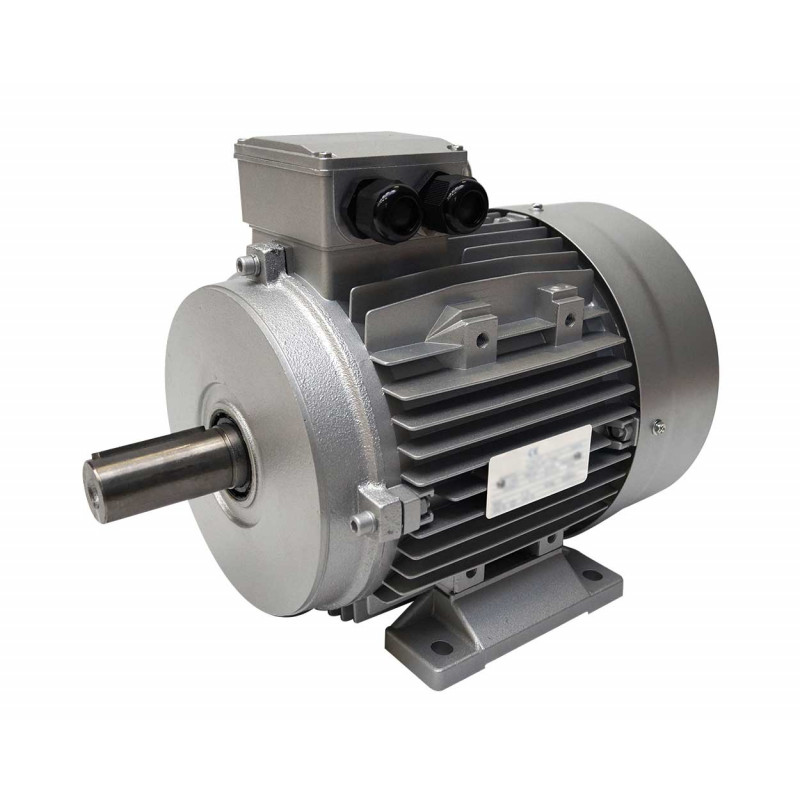
\includegraphics[width=.3\textwidth,height=.4\textheight,keepaspectratio]{images/moteur_electrique_triphase}

	Le moteur à courant continu converti l'énergie électrique en énergie mécanique.
\end{minipage}\hfill
\begin{minipage}[b]{.49\textwidth}
\centering
	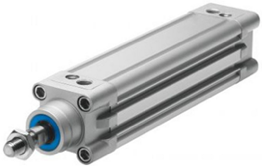
\includegraphics[width=.3\textwidth,height=.4\textheight,keepaspectratio]{images/verin_pneu}

	Un vérin pneumatique converti une énergie pneumatique en énergie mécanique.
\end{minipage}
 %
}

\UPSTIremarque{Les actionneurs ne sont généralement pas reliés directement à l'automate. Un pré-actionneur fait le lien et adapte l'énergie pour l'actionneur.}
